%% abtex2-modelo-include-comandos.tex, v-1.9.6 laurocesar
%% Copyright 2012-2016 by abnTeX2 group at http://www.abntex.net.br/ 
%%
%% This work may be distributed and/or modified under the
%% conditions of the LaTeX Project Public License, either version 1.3
%% of this license or (at your option) any later version.
%% The latest version of this license is in
%%   http://www.latex-project.org/lppl.txt
%% and version 1.3 or later is part of all distributions of LaTeX
%% version 2005/12/01 or later.
%%
%% This work has the LPPL maintenance status `maintained'.
%% 
%% The Current Maintainer of this work is the abnTeX2 team, led
%% by Lauro César Araujo. Further information are available on 
%% http://www.abntex.net.br/
%%
%% This work consists of the files abntex2-modelo-include-comandos.tex
%% and abntex2-modelo-img-marca.pdf
%%

% ---
% Este capítulo, utilizado por diferentes exemplos do abnTeX2, ilustra o uso de
% comandos do abnTeX2 e de LaTeX.
% ---

\chapter{Introdução}\label{intro}

	A vida, como a conhecemos, é totalmente baseada em compostos que são formados estruturalmente por átomos de carbono.  A existência de proteínas, DNA, RNA, lipídeos, carboidratos e outras biomoléculas dependem diretamente da capacidade de formação de ligações químicas fortes e estáveis carbono-carbono e de átomos de carbono com outros átomos, tais como hidrogênio, oxigênio e nitrogênio. Esse fato faz com que o carbono seja considerado diretamente responsável por viabilizar a existência de todas as formas de vida conhecidas no planeta terra.\cite{nelson2008lehninger}
	
	A diversidade estrutural resultante dos diferentes tipos de ligações que o carbono pode fazer resulta em uma miríade de moléculas e estruturas possíveis. Essas estruturas podem apresentar diversas aplicações tecnológicas, abrangendo desde o desenvolvimento de novas moléculas bioativas, como fármacos, até a produção novos materiais sintéticos orgânicos, como polímeros. 

	\begin{figure}[h!]
		\centering
		\includegraphics[width=.7\linewidth]{capitulos/fig/intro/Lascaux_painting.jpg}
		\caption{Pintura rupestre nas cavernas de Lascaux, França. Um dos primeiros usos conscientes do carbono, na forma de carvão, pela humanidade. Fonte: Saxx, P. \textit{Photography of Lascaux animal painting}}
		\label{Lascaux_painting}
	\end{figure}

	Apesar de ser somente o sexto elemento mais abundante no universo \cite{heiserman1991exploring} e o 15$^\circ$ elemento mais abundante na crosta terrestre \cite{morgan1980chemical}, o carbono é conhecido pela humanidade há milênios. Seu nome deriva da palavra em latim \textit{carbo}, traduzida como \textit{carvão} em português, sua principal fonte desde a antiguidade. Um dos primeiros usos conscientes do carbono pela humanidade de que se tem notícia está preservada nas pinturas paleolíticas do complexo de cavernas de Lascaux \cite{leroi1982archaeology}, na vila de Montignac localizada no sudoeste da França. Com uma idade estimada de aproximadamente 17.000 anos \cite{leroi1979datations}, cerca de 600 pinturas representam principalmente a fauna cotidiana dos humanos da era paleolítica. A \autoref{Lascaux_painting}, adaptada de \cite{lascaux}, mostra um exemplo de pintura em que é possível notar claramente a utilização de carbono, na forma de carvão, para desenhar os traços dos animais representados. 
	
	Ao longo da evolução da humanidade, o carbono começou a adquirir um papel cada vez mais central no desenvolvimento tecnológico. Inicialmente era utilizado somente como fonte de energia na forma dos combustíveis como carvão, gás natural e combustíveis fósseis derivados de petróleo. Entretanto, recentemente passou a chamar atenção como fonte de materiais com propriedades eletrônicas, óticas e mecânicas especiais como nanotubos de carbono, fulerenos e o grafeno. 
	
	\section{O átomo de carbono}   
	
	O átomo carbono é composto por 6 prótons, 6 nêutrons e 6 elétrons em sua forma isotópica mais estável \textsuperscript{12}C, que corresponde a aproximadamente 99\% do total de átomos de carbono. Seus outros isótopos se apresentam de maneira muito rara na natureza, sendo o \textsuperscript{13}C aproximadamente 1\% do conteúdo total de átomos e somente traços de \textsuperscript{14}C compondo aproximadamente 1/$10^{12}$ de todos os átomos de carbono. 
	
	Apesar de sua pouca incidência na natureza, ambos os isótopos apresentam aplicações muito importantes. O \textsuperscript{13}C é amplamente utilizado em experimentos de ressonância magnética nuclear, por possuir spin nuclear 1/2. O \textsuperscript{14}C é utilizado para datação histórica de objetos, fósseis antigos ou quaisquer compostos que contenham átomos de carbono, pois como seu tempo de meia vida é de aproximadamente 5700 anos, o que representa um tempo considerável para a história humana, e a taxa de incorporação deste isótopo em materiais biológicos ou feitos pelos humanos é aproximadamente constante. Dessa forma pode-se usar a quantidade de \textsuperscript{14}C ainda presente em uma amostra para determinar seu tempo de vida. 
	
	Em seu estado fundamental, que apresenta termo espectroscópico $^3$P$_0$ \cite{johansson1966spectrum}, seus 6 elétrons se apresentam em uma configuração eletrônica 1s$^2$2s$^2$2p$^2$: $1s$ \framebox[.25in]{$\upharpoonleft \downharpoonright$} $2s$ \framebox[.25in]{$\upharpoonleft \downharpoonright$}  $2p_x$ \framebox[.25in]{$\upharpoonleft$} $2p_y$ \framebox[.25in]{$\upharpoonleft$} $2p_z$ \framebox[.25in]{\color{white}$\upharpoonleft$}. Nessa forma, somente os elétrons desemparelhados $2p_x$ e $2p_y$ estão disponíveis para a formação de ligações químicas e, portanto, cada átomo carbono só poderia, em princípio, fazer no máximo duas ligações químicas. 
	
	Entretanto, é necessário somente 1.6 eV para excitar o átomo de carbono para o estado $^5$S$_2$ com configuração 1s$^2$2s$^1$2p$^3$:  $1s$ \framebox[.25in]{$\upharpoonleft \downharpoonright$} $2s$ \framebox[.25in]{$\upharpoonleft$}  $2p_x$ \framebox[.25in]{$\upharpoonleft$} $2p_y$ \framebox[.25in]{$\upharpoonleft$} $2p_z$ \framebox[.25in]{$\upharpoonleft$}, contendo quatro elétrons desemparelhados e, dessa forma, podendo fazer um total de quatro ligações químicas. Como os orbitais 2p ($2p_x$, $2p_y$ e $2p_z$) são aproximadamente 4 eV mais energéticos do que o orbital 2s (\autoref{carbon_hibrid}), para um átomo isolado é energeticamente mais favorável que dois elétrons ''preencham'' o orbital 2s e os outros 2 ''preencham'' dois orbitais 2p. Na presença de outros átomos, como hidrogênio, oxigênio ou até mesmo outro átomo de carbono, o ganho de energia pela formação de uma ligação química supera a diferença de energia entre os orbitais 2s e 2p, fazendo com que essa alteração em sua estrutura eletrônica seja energeticamente favorecida. 

	
	\section{Hibridizações do carbono}
	
		
	\begin{figure}[!h]
		\centering
		\includegraphics[width=1.\linewidth]{capitulos/fig/intro/hibrid_carbon.pdf}
		\caption{Representação esquemática da formação de orbitais híbridos do carbono.}
		\label{carbon_hibrid}
	\end{figure}

	As considerações energéticas explicam o fato de o carbono conseguir fazer 4 ligações, apesar de o estado fundamental do átomo isolado apresentar somente dois elétrons desemparelhados. Entretanto, ainda há dois tipos de orbitais diferentes, $s$ e $p$, que resultarão na formação de dois tipos de ligações diferentes. Entretanto, dados experimentais mostram que as ligações químicas em moléculas como o metano (CH\textsubscript{4}) apresentam exatamente a mesma energia. Além disso, a formação de ligações dos orbitais $s$ do hidrogênio com os orbitais $s$ ou $p$ do carbono não poderiam gerar uma molécula com geometria tetraédrica, como é a apresentada por essa molécula.
	
	Outro fator importante que deve ser levado em consideração é que a transição $^3$P$_0 \rightarrow ^5$S$_2$ é proibida segundo as regras de seleção\footnote{Somente transições eletrônicas com $\Delta J = 0, \pm 1$ e $\Delta S = 0$ são permitidas, onde $\Delta J$ e $\Delta S$ são as variações de momento angular total e spin total}. Todos estes detalhes fazem com que um novo modelo deva ser proposto para explicar os dados experimentais observados.
	
	Um modelo desenvolvido para explicar esses fenômenos foi proposto em \citeyear{pauling1931nature} por \citeauthor{pauling1931nature}, conhecido como modelo de orbitais híbridos. Esse modelo prevê que os orbitais \textit{s} e \textit{p}, que podem ser representados no formalismo quanto-mecânica na forma $|2s\rangle$, $|2p_x\rangle$, $|2p_y\rangle$ e $|2p_z\rangle$, podem se combinar linearmente para formar um estado sobreposto, chamado de estado híbrido. Nesse processo, um estado $|2s\rangle$ pode se combinar com $n$ estados $|2p_j\rangle$, sendo $n$=1, 2 ou 3, formando orbitais híbridos do tipo $sp^n$, como esquematizado na \autoref{carbon_hibrid}.
	
	\subsection{Hibridização \textit{sp}}
	
		Um átomo que possui orbitais $|2s\rangle$ e $|2p\rangle$ pode combinar linearmente estes orbitais para formar novos orbitais híbridos na forma
		
		\begin{subequations}
			\label{sp1hibrid}
			\begin{flalign}
			\phi_1& = \frac{1}{2}|2s\rangle + \frac{1}{2}|p_x\rangle\\
			\phi_2& = \frac{1}{2}|2s\rangle - \frac{1}{2}|p_x\rangle\\
			\phi_2& = |p_y\rangle \\
			\phi_4& = |p_z\rangle
			\end{flalign}
		\end{subequations}
	
		Quando ocorre a combinação de um orbital $2s$ com um orbital $2p$, o resultado é a formação de dois orbitais híbridos $sp$, $\phi_1$ e $\phi_2$, com ângulos de 180$^\circ$ em uma formato linear, como mostrado na \autoref{carbon_hibrid}. Após a formação dos orbitais híbridos $sp$ ainda restam dois orbitais do tipo $p$, possibilitando assim formação de duas ligações $\sigma$, resultando da sobreposição frontal dos orbitais $sp$ com orbitais de outro átomo, e duas ligações $\pi$, resultando da sobreposição lateral destes orbitais com os orbitais $p$ de outro átomo. Consequentemente, pode ocorrer a formação ou de uma ligação tripla, como a apresentada pelo acetileno, ou duas ligações duplas, como apresentada em cumulenos.\footnote{É importante ressaltar que aqui e ao longo de toda esta dissertação as denominações de ligações $\sigma$ e $\pi$ estão sendo usadas para se referir às ligações formadas por sobreposição frontal e lateral dos orbitais, respectivamente, e não para se referir à sua definição estrita como sendo o valor da projeção do momento angular no eixo da ligação.}

	\subsection{Hibridização \textit{sp\textsuperscript{2}}}
	
		Os orbitais $|2s\rangle$ e $|2p\rangle$ também podem ser combinados para formar novos orbitais híbridos na forma
		
		\begin{subequations}
			\label{sp2hibrid}
			\begin{flalign}
				\phi_1& = \frac{1}{\sqrt{3}}|2s\rangle + \frac{\sqrt{2}}{\sqrt{3}}|p_x\rangle\\
				\phi_2& = \frac{1}{\sqrt{3}}|2s\rangle - \frac{1}{\sqrt{6}}|p_x\rangle +  \frac{1}{\sqrt{2}}|p_y\rangle \\
				\phi_2& = \frac{1}{\sqrt{3}}|2s\rangle - \frac{1}{\sqrt{6}}|p_x\rangle -  \frac{1}{\sqrt{2}}|p_y\rangle \\
				\phi_4& = |p_z\rangle
			\end{flalign}
		\end{subequations}
		
		Os três primeiros orbitais, $\phi_1$, $\phi_2$ e $\phi_3$, apresentam uma distribuição espacial trigonal e ângulos intrínsecos de 120$^\circ$, como mostrado na \autoref{carbon_hibrid}, podendo formar três ligações $\sigma$. O orbital $\phi_4$ aponta para a direção perpendicular ao plano $xy$, e pode formar uma ligação $\pi$. Como esses orbitais são compostos por um estado $s$ e 2 estados $p$ cada, recebem o nome de orbitais híbridos $sp^2$. Esses orbitais apresentam a mesma energia ($\epsilon_s + 2\epsilon_p$)/3, onde $\epsilon_s$ e $\epsilon_p$ são as energias dos estados $s$ e $p$ respectivamente.
	
	\subsection{Hibridização \textit{sp\textsuperscript{3}}}
	
		Os orbitais $|2s\rangle$ e $|2p\rangle$ também podem ser combinados na forma
		
		\begin{subequations}
			\label{sp3hibrid}
			\begin{flalign}
			\phi_1& = \frac{1}{2}\left[|2s\rangle - |p_x\rangle - |p_y\rangle - |p_z\rangle\right]\\
			\phi_2& = \frac{1}{2}\left[|2s\rangle + |p_x\rangle - |p_y\rangle + |p_z\rangle\right]\\
			\phi_2& = \frac{1}{2}\left[|2s\rangle + |p_x\rangle + |p_y\rangle - |p_z\rangle\right]\\
			\phi_4& = \frac{1}{2}\left[|2s\rangle - |p_x\rangle + |p_y\rangle + |p_z\rangle\right]
			\end{flalign}
		\end{subequations}
		
		Esses novos estados formados recebem o nome de $sp^3$, pois são formados pela combinação de 1 orbital $s$ com 3 orbitais $p$. Esses orbitais apontam do centro para os vértices de um tetraedro, como mostrado na \autoref{carbon_hibrid}, com ângulos intrínsecos de 108$^\circ$ e apresentando todos a mesma energia de ($\epsilon_s + 3\epsilon_p$)/4, podendo formar quatro ligações $\sigma$. 
		 
	\section{Formas Alotrópicas do Carbono}

	\begin{figure}[!ht]
		\centering
		\includegraphics[width=.7\linewidth]{capitulos/fig/intro/alotropos_carbono}
		\caption{Representação geral das diversas estruturas que podem ser formadas a partir da combinação carbonos com diferentes hibridações. }
		\label{carbon_alotropes}
	\end{figure}
	
	Alótropos são definidos como os vários arranjos estruturais de um único elemento \cite{mcnaught1997compendium}. Graças à diversidade estrutural possibilitada pela formação de orbitais híbridos, o carbono possui uma quantidade muito grande de estruturas alotrópicas relatadas. Existe uma quantidade relativamente grande de alótropos de carbono já observados experimentalmente, como por exemplo: grafite, diamante, Lonsdaleite, nanotubos, fulerenos, grafeno, carbino, entre outras. Essas formas e sua ligação com a hibridização estão representadas na \autoref{carbon_alotropes} (Fonte: Adaptado de \cite{stauss2017diamondoids}). 
	
	Além das que já foram observadas experimentalmente, há uma diversidade grande de estruturas hipotéticas já estudadas. De acordo com o banco de dados \textbf{Samara Carbon Allotrope Database (SACADA)} em 2019 já existiam mais de 500 estruturas, hipotéticas ou observadas experimentalmente, relatadas \cite{hoffmann2016homo}. A \autoref{carbon_alotropes} apresenta os alótropos de carbono obtidos experimentalmente agrupados pela hibridação dos átomos que os constitui. É interessante notar que algumas estruturas como Cyclo[18]carbon, fulerenos e nanotubos apresentam átomos com geometria intermediária entre as canônicas $sp^n$, mostrando que apesar de explicar satisfatoriamente grande parte dos dados experimentais a teoria de hibridação de Pauling não deve ser tomada como absoluta e ainda apresenta espaço para ser melhorada. 

	A observação experimental do fulereno em \citeyear{kroto1985c60} por \citeauthor{kroto1985c60}, dos nanotubos de carbono em \citeyear{iijima1991helical} por \citeauthor{iijima1991helical} e do grafeno em \citeyear{novoselov2004electric} por \citeauthor{novoselov2004electric} iniciou uma era sem precedentes de descobertas e proposições de novos alótropos de carbono. Essas descobertas foram tão impactantes que renderam o prêmio Nobel de Química em 1996\cite{prato199760} para Robert F. Curl, Sir Harold W. Kroto e Richard E. Smalley pela observação dos fulerenos e o prêmio Nobel de Física em 2010 \cite{gerstner2010nobel} para Andre Geim e Konstantin Novoselov pela descoberta do grafeno, antecipando a grande importância que este material teria no desenvolvimento da ciência e tecnologia futura. 
	
	Juntas, essas descobertas encorajaram pesquisadores das diversas áreas da ciência a buscar tanto a observação experimental quanto a predição teórica de novos alótropos de carbono que apresentem propriedades óticas, eletrônicas e mecânicas excepcionais \cite{taylor1992third}, fazendo com que muitos considerem esse momento como a "Era dos alótropos de carbono" \cite{neto2010carbon, hirsch2010era}.
		
	\begin{figure}[!h]
		\centering
		\subfloat{\includegraphics[width=.45\linewidth]{capitulos/fig/intro/publica_carbon_allotropes}}
		\subfloat{\includegraphics[width=.45\linewidth]{capitulos/fig/intro/publica_carbon_allotropes_t}} 
		\caption{Número de publicações contendo o termo "carbon allotrope" no artigo à esquerda e no título à direita. Fonte: Google Scholar acessado em 10/01/2020}
		\label{public}
	\end{figure}
	
	De fato, uma busca por artigos publicados em periódicos científicos com revisão por pares pelo termo "carbon allotrope", apresentada na \autoref{public}, mostra um crescimento exponencial por menções à esse tema indicando sua crescente relevância acadêmica. É possível notar também que o número de publicações que apresentam esse termo no título, como é comum para artigos que apresentam novos alótropos de carbono, apresenta uma quantidade bem pequena. Isso indica que apesar do interesse muito grande em alótropos de carbono, o número de novas estruturas relatadas é relativamente pequeno. 
	
	Recentemente a observação experimental do cyclo[18]carbon por \citeauthor{kaiser2019sp} em \citeyear{kaiser2019sp} trouxe uma nova onda de interesse em materiais formados somente por átomos de carbono. Essa forma alotrópica já havia sido predita por \citeauthor{diederich1992synthetic} em \citeyear{diederich1992synthetic}, que também apresentaram uma possível rota sintética para sua obtenção. Vinte e sete anos depois essa rota sintética proposta foi utilizada para trazer esse alótropo à realidade, mostrando o poder e a importância que cálculos teóricos possuem na descoberta de novas estruturas. 
	
	Nesta dissertação será apresentado e explorado o uso de cálculos teóricos de estruturas alotrópicas de carbono, a fim de buscar um entendimento de sua capacidade preditiva e ampliar a gama de materiais formados unicamente por átomos de carbono.
	
	
\chapter{Revisão Bibliográfica}

	\section{Busca computacional por novos alótropos: Início da história}

		Obter a estrutura molecular de um material é um ponto chave para se entender a fundo suas diversas propriedades. Uma das primeiras sugestões de estruturas alotrópicas hipotéticas foi feita por \citeauthor{gibson194687} em \citeyear{gibson194687} e \citeauthor{riley1950chemical} em \citeyear{riley1950chemical}, na tentativa de propor uma estrutura para materiais pirolíticos carbonáceos. A \autoref{alotropos_hip}-\textbf{a} apresenta a estrutura proposta por Gibson, Holohan e Riley. Apesar de nenhum tipo de cálculo ter sido feito, a ideia de imaginar novas estruturas compostas somente por átomos de carbono despertou a imaginação de diversos pesquisadores.
		
			
		\begin{figure}[!h]
			\centering
			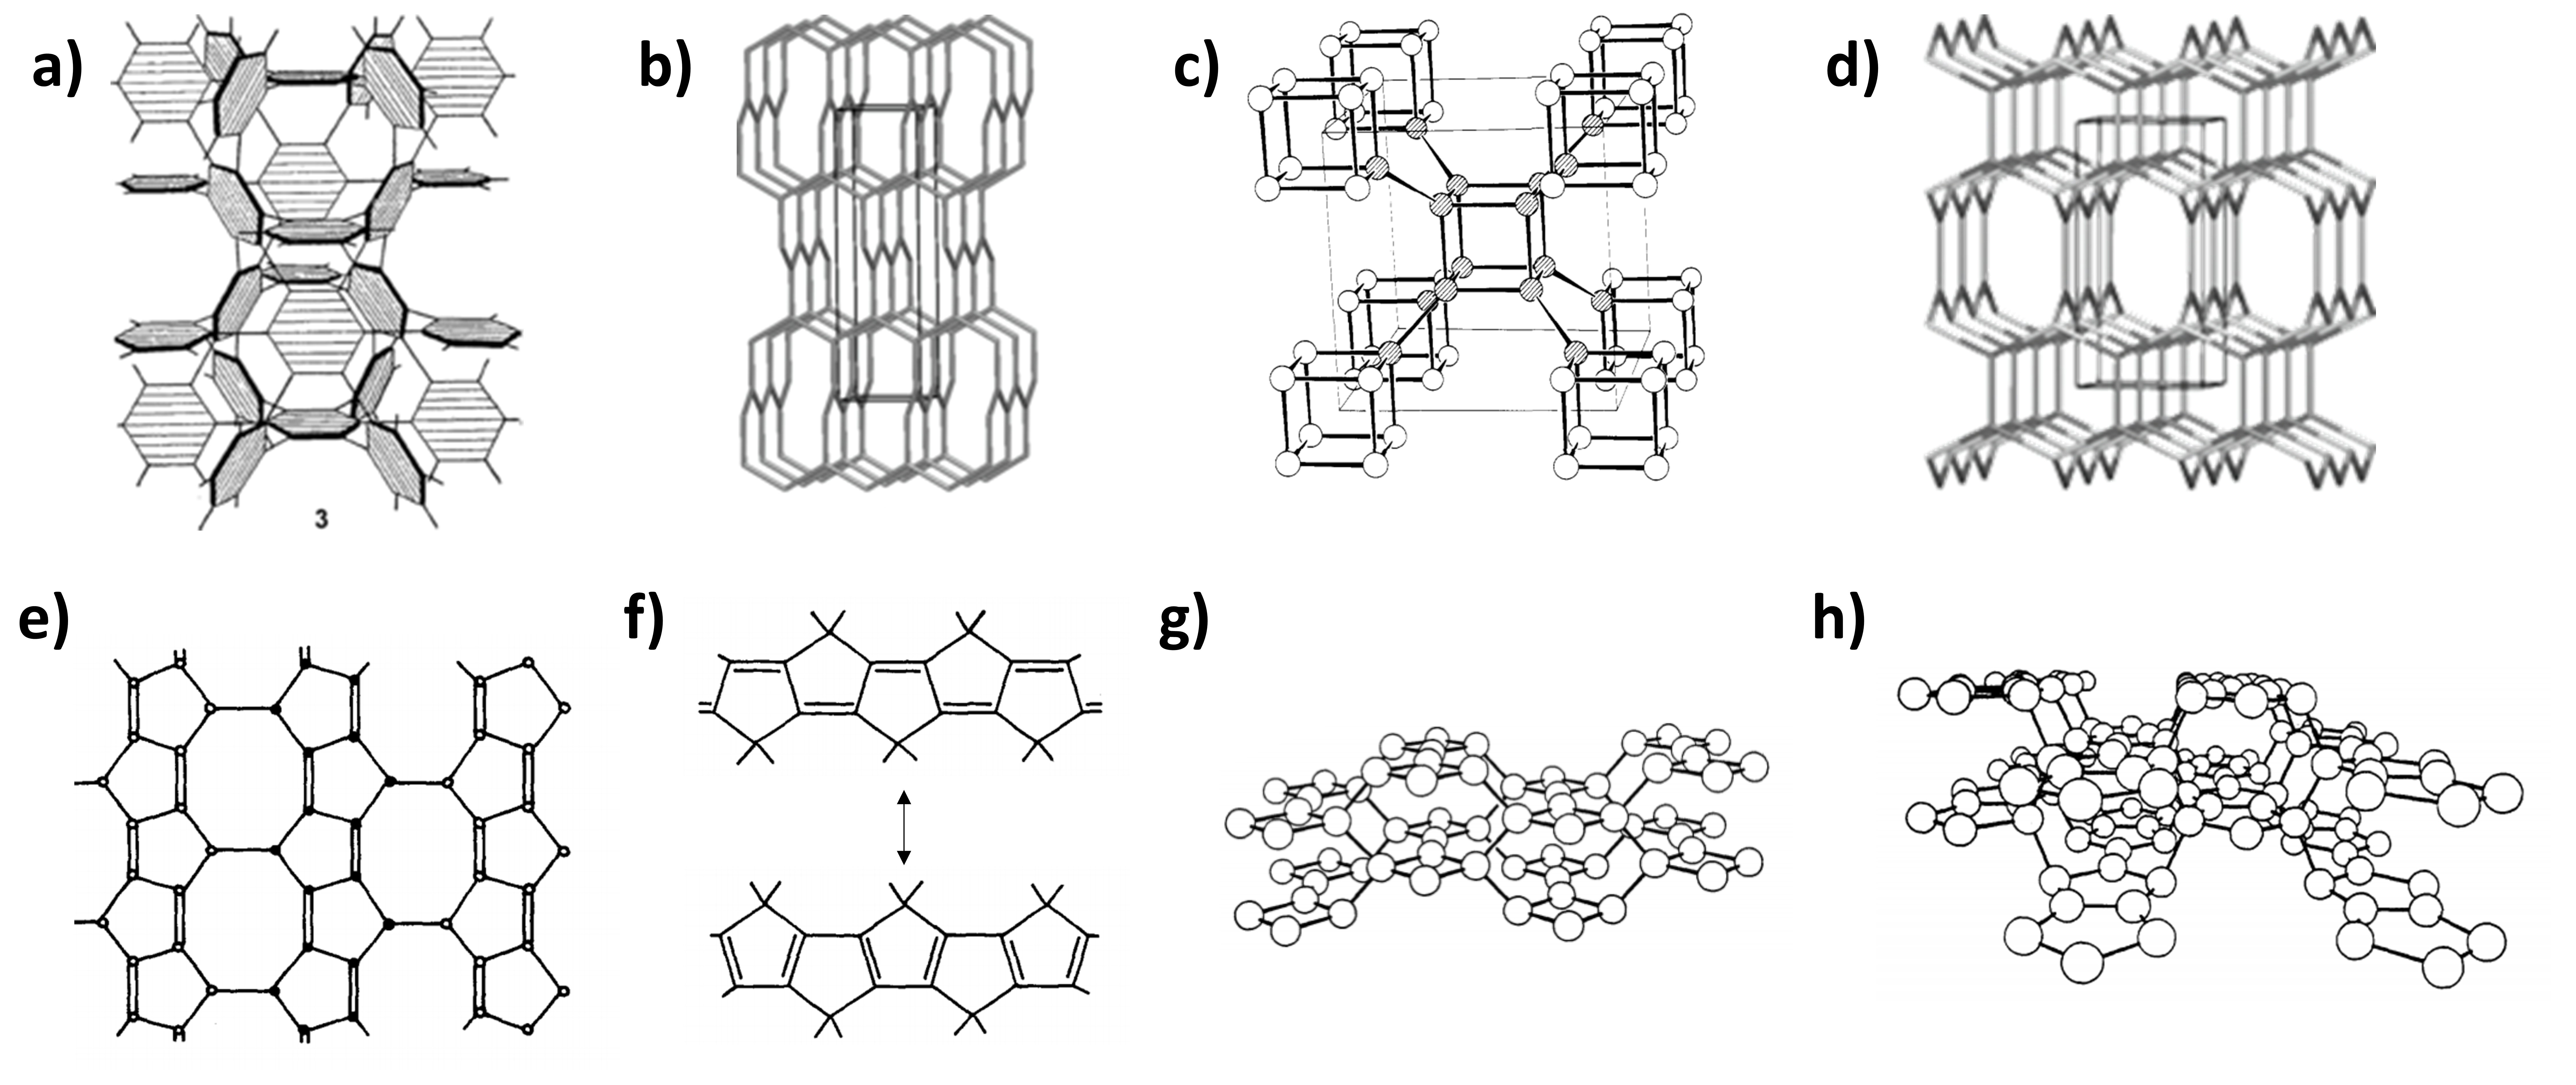
\includegraphics[width=1\linewidth]{capitulos/fig/intro/alotropos_hipoteticos}
			\caption{Representação de diversas estruturas alotrópicas hipotéticas propostas para o carbono.}
			\label{alotropos_hip}
		\end{figure}
	
		Com o advento e popularização dos cálculos de estrutura eletrônica a partir da década de 1980, diversas formas alotrópicas puramente hipotéticas puderam ter sua estrutura e suas propriedades exploradas. Um dos primeiros trabalhos desse tipo foi publicado por \citeauthor{hoffmann1983hypothetical} em \citeyear{hoffmann1983hypothetical}\footnote{Em seu artigo original Hoffmann não apresenta detalhes da metodologia computacional utilizada}, onde foi apresentada uma nova estrutura - chamada posteriormente de \textbf{bct-4} - composta somente por átomos de carbono $sp^2$ formando um novo alótropo de carbono metálico, com uma célula unitária tetragonal com grupo espacial \textit{I4\textsubscript{1}/amd} e grupo pontual $D^{19}_{4h}$ em uma rede 3-c $10^3$-\textbf{ths}\footnote{Seguindo a notação de redes periódicas proposta por \citeauthor{o2008reticular}} (\autoref{alotropos_hip}-\textbf{b}). Em \citeyear{johnston1989superdense} uma outra forma alotrópica, denominada \textbf{C\textsubscript{8}} foi proposta sendo formada por átomos de carbono formando cubos conectados pelo vértice (\autoref{alotropos_hip}-\textbf{c}), gerando um alótropo de carbono com alta densidade (0.338 mol/cm$^3$ contra 0.295 mol/cm$^3$ para o diamante). Em \citeyear{bucknum1994hypothetical} mais uma estrutura foi proposta por \citeauthor{bucknum1994hypothetical}, sendo formada por unidades 1,4-ciclohexadienoides em uma rede 3,4-c \textbf{tfi}, denominada spirographite (\autoref{alotropos_hip}-\textbf{d}). 
	
		Em \citeyear{balaban1989carbon} \citeauthor{balaban1989carbon} publicou um extenso trabalho explorando aspectos estruturais e da simetria de diversas estruturas alotrópicas de carbono. Nesse trabalho ele analisou as possíveis propriedades eletrônicas e propôs maneiras de nomear as diversas estruturas resultantes baseando-se na teoria de grafos, resultando em um belo sinergismo entre química e matemática. Esse trabalho pioneiro mostrou matematicamente que, devido às diferentes hibridações possíveis do átomo de carbono, o número de estruturas alotrópicas geradas pela combinação dessas diferentes formas é extremamente grande. Algumas das estruturas propostas por \citeauthor{balaban1989carbon} estão representadas na \autoref{alotropos_hip}-\textbf{e-h}.
		
		Diederich em \citeyear{diederich1992synthetic} \cite{diederich1992synthetic} e \citeyear{diederich1994carbon} \cite{diederich1994carbon, diederich1994synthetic} fez importantes contribuições à classe de novos alótropos de carbono. Através de uma meticulosa revisão da literatura e propostas criativas de novas estruturas, Diederich ajudou a construir uma biblioteca de reações que podem ser capazes de trazer diversas estruturas hipotéticas à realidade. De fato esse trabalho foi especialmente importante na preparação e observação do cyclo[18]carbon\cite{kaiser2019sp}, o mais recente alótropo de carbono relatado na literatura, demonstrando que a predição teórica da novas estruturas pode levar a sua futura obtenção experimental.
		
		Os trabalhos de Hoffmann, Balaban e Diederich abriram caminho e serviram como base e inspiração para que diversos pesquisadores investissem na busca computacional de novas estruturas alotrópicas, o foco principal do presente trabalho.
	
	\section{Alótropos com alta dureza}
	
		O diamante é conhecido principalmente por sua elevada dureza, sendo o material natural mais duro conhecido. Essa propriedade é resultado do tipo e natureza das ligações entre os átomos deste sólido. As ligações do tipo covalente são, em geral, muito mais fortes do que as apresentadas nos sólidos iônicos, e a geometria das ligações faz com que qualquer força em um átomo seja distribuída espacialmente para outros três átomos de maneira simétrica. Sua dureza medida na escala de Vickers é de 96$\pm$5 GPa e seu módulo Bulk é 443 GPa \cite{andrievski2001superhard}.  Inspirado no diamante, muitas pesquisas têm sido feitas na busca por novas estruturas de carbono com dureza próxima ou maior. 
				
		\begin{figure}[!h]
			\centering
			\includegraphics[width=.7\linewidth]{capitulos/fig/intro/superhard}
			\caption{Representação esquemática das estruturas de (a) bct-C$_4$, (b) M-Carbon, (c) T-Carbon, (d) W-Carbon e (e) Cco-C$_8$}
			\label{superhard}
		\end{figure}
	
		Em \citeyear{li2009superhard} \citeauthor{li2009superhard} identificaram a estrutura hipotética de um alótropo monoclínico com grupo espacial $C2/m$ utilizando busca evolucionária estrutural \cite{oganov2006crystal}. Essa estrutura, denominada M-Carbon, \autoref{superhard}-\textbf{b}, apresenta módulo Bulk calculado de 431.2 GPa e dureza calculada de 83.1 GPa, valores próximos do apresentado pelo diamante. 
		
		Em \citeyear{umemoto2010body} \citeauthor{umemoto2010body} identificaram mais uma fase cristalina composta somente por átomos de carbono com hibridação $sp^3$ a partir de simulações de dinâmica molecular da compressão de nanotubos de carbono do tipo (2,2). A estrutura resultante, denominada bct C$_4$, \autoref{superhard}-\textbf{a}, apresenta uma célula unitária tetragonal de corpo centrado com grupo pontual $I_4/mmm$ e módulo Bulk calculado de 428.7 GPa.
		
		Em \citeyear{wang2011low} \citeauthor{wang2011low} propuseram a estrutura de um alótropo ortorrômbico de corpo centrado com grupo espacial $Pmna$ e grupo pontual $D^{16}_{2h}$. Essa estrutura denominada W-Carbon, \autoref{superhard}-\textbf{d}, apresenta módulo Bulk de 444.5 GPa. No mesmo ano \citeauthor{zhao2011novel} propuseram a estrutura de um alótropo ortorrômbico de corpo centrado com grupo espacial $Cmmm$. Essa estrutura, denominada Cco-C\textsubscript{8} (\autoref{superhard}-\textbf{e}) é composta somente por átomos de carbono $sp^3$ e apresenta dureza calculada de 95.1 e módulo Bulk de 441 GPa. 
		
		Ainda em \citeyear{sheng2011t} \citeauthor{sheng2011t} propuseram a formação de um novo alótropo de carbono substituindo cada átomo de carbono da estrutura do diamante por uma unidade derivada de um tetraedrano, molécula hipotética em que cada vértice de um tetraedro é um átomo de carbono, formando o T-Carbon (\autoref{superhard}-\textbf{c}). A estrutura resultante se apresenta em uma célula unitária cúbica de corpo centrado com grupo pontual Fd$\bar{3}$m, possuindo módulo Bulk calculado de 169 GPa e dureza de 61.1 GPa. Esse alótropo foi obtido experimentalmente em \citeyear{zhang2017pseudo} por \citeauthor{zhang2017pseudo} através da conversão de nanotubos de carbono irradiados por laser e por \citeauthor{xu2020preparation} em \citeyear{xu2020preparation} através de deposição química de vapor (CVD). Esse é mais um ótimo exemplo de como a busca computacional de novos alótropos pode incentivar e guiar sua obtenção experimental.
		
		Em \citeyear{tian2012superhard} \citeauthor{tian2012superhard} utilizaram uma metodologia de otimização do tipo "\textit{particle-swarm}" para obter a estrutura hipotética de um alótropo monoclínico com simetria P2/m (C$^{1}_{2h}$). Essa estrutura, denominada F-Carbon (\autoref{superhard}-\textbf{f}) é composta somente por átomos de carbono sp$^3$ e apresenta dureza calculada de 93.9 GPa e módulo Bulk de 410 GPa.
		
		Com o avanço do tempo e a crescente atenção dada a essas estruturas, muitos grupos começaram a investir em generalizar conceitos e criar famílias de novos alótropos. \citeauthor{niu2012families} propuseram uma família composta por P-, R- e S-Carbon. 
	
	\section{Alótropos com propriedades eletrônicas especiais}
	
		Em \citeyear{baughman1987structure} \citeauthor{baughman1987structure} propuseram a existência de um conjunto de alótropos de carbono lamelares, sendo formados por átomos com hibridações $sp^2$ e $sp$. Esse é um dos primeiros exemplos de aplicação de uma regra estrutural sistemática na construção de estruturas estendidas. A estratégia principal é de substituir as ligações entre os anéis benzênicos ou entre as ligações duplas do grafite por unidades acetilênicas (-C$\equiv$C-), gerando três estruturas denominadas $\alpha$, $\beta$ e $\gamma$ grafino\footnote{Traduzindo livremente do original em inglês \textit{graphyne}}. Algumas dessas estruturas já haviam sido preditas em \citeyear{balaban1968chemical} por \citeauthor{balaban1968chemical}, porém não foram exploradas profundamente. O conceito do grafino pode ser generalizado considerando a substituição das ligações entre os anéis benzênicos do grafite por $n$ unidades acetilênicas, gerando assim a família dos $n$-grafinos. O 2-grafino, também chamado de grafidiino, foi sintetizado em \citeyear{li2010architecture} por \citeauthor{li2010architecture}.
		
		\citeauthor{baughman1987structure} consideraram em seus cálculos uma estrutura tridimensional lamelar, como a do grafite. Apesar de essa ser a forma mais estável para esses alótropos, após a observação experimental do grafeno uma corrida foi iniciada pela descoberta de novas estruturas bidimensionais com propriedades extraordinárias. \citeauthor{kim2012graphyne} mostraram através de cálculos DFT e \textit{tight-binding} que  $\alpha$- e $\beta$-1-grafino (\autoref{graphyne}-b e c) apresentam cones de Dirac em seu diagrama de bandas, com velocidades de Fermi dos elétrons próximas ao apresentado pelo grafeno. O $\gamma$-1-grafino (\autoref{graphyne}-d) apresenta um \textit{band gap} pequeno, de aproximadamente 0.47 eV, que diminui com o aumento do comprimento da ligação tripla e chega à zero quando o comprimento é de 1.278 Å.
		
		\begin{figure}[!h]
			\centering
			
\includegraphics[width=1\linewidth]{capitulos/fig/intro/graphyne}
			\caption{Representação esquemática e diagrama de bandas de (a) Grafeno, (b) $\alpha$-1-grafino, (c) $\beta$-1-grafino e (d) $\gamma$-1-grafino, (e) 6,6,12-grafino.}
			\label{graphyne}
		\end{figure}
	
		Uma quarta variante dessa estrutura explorada por \citeauthor{malko2012competition} em \citeyear{malko2012competition}, o 6,6,12-grafino (\autoref{graphyne}-e), apresenta dois cones de Dirac \footnote{Quando materiais apresentam bandas de valência e de condução se cruzando de maneira que lembra um cone em energias próximas do nível de Fermi ele pode apresentar propriedades eletrônicas especiais. Esse cruzamento recebe o nome de cone de Dirac.} em seu diagrama de bandas, um primeiro levemente abaixo do nível de Fermi e um segundo logo acima do nível de Fermi.\cite{malko2012competition} Esse fenômeno é resultado de uma auto-dopagem, no sentido de que no primeiro cone os elétrons se apresentam como portadores de carga e no segundo os buracos se apresentam como portadores de carga. Além disso, os cones apresentam formatos diferentes, indicando que as propriedades eletrônicas devido à esse fenômeno podem apresentar dependência direcional. 
		
		Outra curiosidade interessante é que a incidência de cones de Dirac está fortemente relacionada com estruturas que apresentam simetria hexagonal (p6m)\cite{wehling2014dirac}, entretanto essa estrutura apresenta dois cones de Dirac mesmo possuindo simetria retangular (pmm).
		
		A busca por propriedades eletrônicas excepcionais se estendeu além da procura por férmions topológicos de Dirac em sistemas 2D, tendo recentemente crescido na direção de fases topológicas exóticas como isolantes topológicos (materiais em que o \textit{Bulk} é isolante mas as bordas são condutoras), \textit{"nodal loop semimetals"} (sistemas 3D onde as bandas de valência e condução se tocam em \textit{loops} fechados e espaço dos momentos), ou \textit{"nodal point semimetals"} (materiais onde a superfície de Fermi possui dimensão zero e é conectada por arcos de Fermi na superfície da zona de Brillouin).  
		
		%\begin{figure}[!h]
			%\centering
			%
\includegraphics[width=1\linewidth]{capitulos/fig/intro/topologicos_3D}
			%\caption{Representação esquemática e diagrama de bandas de (a) %Pentagon-Carbon, (b) $\alpha$-1-grafino, (c) $\beta$-1-grafino e (d) %$\gamma$-1-grafino, (e) 6,6,12-grafino.}
		%	\label{topologicos_3d}
		%\end{figure}
		
		Em \citeyear{zhong2017three} \citeauthor{zhong2017three}  apresentaram uma fase metaestável tridimensional composta por anéis pentagonais de carbono conectados perpendicularmente. Essa estrutura, que apresenta grupo espacial \textit{I4\textsubscript{1}/amd} e grupo pontual $D^{19}_{4h}$, já havia sido imaginada por \citeauthor{balaban1989carbon}, porém não havia até então tido sua estrutura eletrônica explorada de maneira mais profunda. Em seu trabalho, os autores mostraram que esse material apresenta férmions topológicos emergentes, no qual quando aplicando-se uma deformação na estrutura o Pentagon Carbon apresenta uma transição de fase topológica passando de férmions tripleto isospin-1 para férmions triplamente degenerados e para férmions do tipo Hopf-link Weyl-loop.
	
	\section{Outras estruturas 3D}
	
		O conceito de inserir unidades do tipo -C$\equiv$C-, utilizando para a idealização dos $n$-grafinos, foi explorado também de maneira independente por \citeauthor{jo2012carbon} em \citeyear{jo2012carbon} para propor a estrutura do Y-Carbon e híbridos entre o Y-Carbon e o T-Carbon, através da inserção de uma unidade de acetileno entre cada átomo de carbono da estrutura do diamante, e por \citeauthor{balaban2013expanded} em \citeyear{balaban2013expanded} para criar uma miríade de estruturas hipotéticas, combinando diversos motivos estruturais. Em \citeyear{costa2018n} nosso grupo também fez uma importante contribuição, generalizando o conceito da inserção de $n$ unidades de acetileno entre os átomos $sp^3$ do diamante e criando a família dos $n$-diamantinos\cite{costa2018n}, sendo o Y-Carbon um membro dessa família denominado 1-diamantino. 
	

	
	
	


